\appendix
\section{Appendix}
\setbeamertemplate{footline}{
  \hfill Appendix \insertframenumber\hspace{1em}\vspace{1ex}
}

\begin{frame}
	\frametitle{Optimization Process}
	\begin{itemize}
		\item Prioritize requirements by model validity
		\item Enforce high-priority requirements with bounds or linear constraints
		\item Sequential quadratic programming + pattern search
		\item Epsilon-constraint seeds to leverage gradients in multi-objective
		      
		\item McCabe, Dietrich, and Haji. “Leveraging Multidisciplinary Design Optimization to Advance Wave Energy Converter Viability.” In preparation for submission to Renewable Energy.
	\end{itemize}
	
\end{frame}


\begin{frame}
	\frametitle{Reduced Order Model}
	
	\centering
	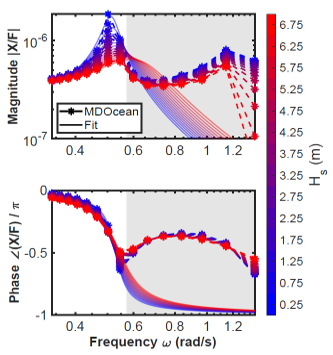
\includegraphics[width=0.9\linewidth]{figs/img0034.png}
	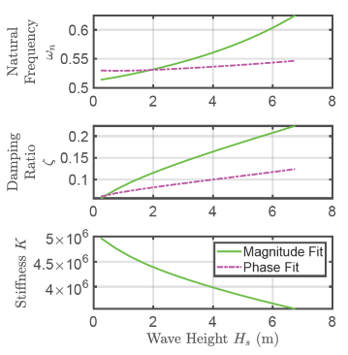
\includegraphics[width=0.9\linewidth]{figs/img0035.png}
	
	{\footnotesize McCabe, Dietrich, Yang, Long, Kuan, Buccino, Liu, and Haji. “WEC optimization to maximize grid economic value and avoided emissions.” University Marine Energy Community Conference, August 2025, Corvallis OR.}
	
\end{frame}


\begin{frame}
	\frametitle{Environmental: LCA Module}
	
	\centering
	\begin{itemize}
		\item Eco-Value: carbon emissions avoided from CEM
		\item Eco-Cost: embodied carbon of steel (dominant), fiberglass, maintenance vessel fuel
		\item Note: if eco-value dominates eco-cost, econ and enviro metrics will not conflict
	\end{itemize}
	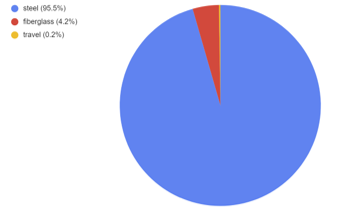
\includegraphics[width=0.9\linewidth]{figs/img0036.png}
	
\end{frame}


\begin{frame}
	\frametitle{Grid Capacity Expansion Model}
	
	\centering
	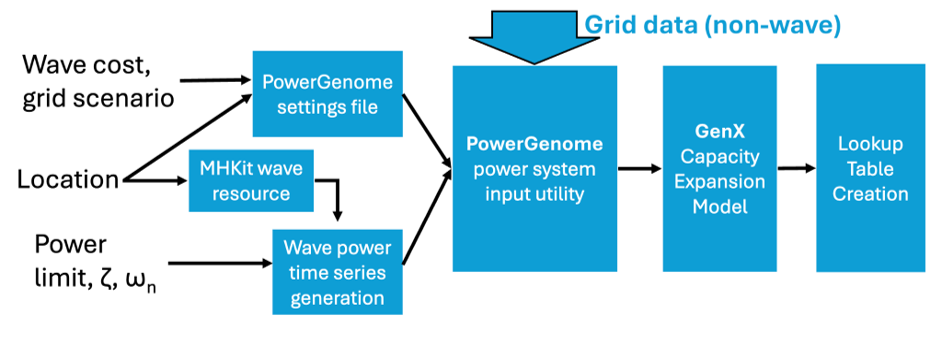
\includegraphics[width=0.9\linewidth]{figs/img0037.png}
	
	{\footnotesize McCabe, Dietrich, Yang, Long, Kuan, Buccino, Liu, and Haji. “WEC optimization to maximize grid economic value and avoided emissions.” University Marine Energy Community Conference, August 2025, Corvallis OR.}
	
\end{frame}


\begin{frame}
	\frametitle{Expected results}
	
	\centering
	\begin{itemize}
		\item Show trend: CA vs northeast vs grid scenario correlation with sea state, and what that means for wec optimization
		\item Where in the power matrix you prioritize when optimizing cost vs value, and econ vs environ, and how this might affect wec design (ie decisions of whether to sit out the winter waves / survive them)
		\item Seasonal complementarity with solar and demand
		      \begin{itemize}
		      	\item Wec produces when price is high so generates more revenue - WEC-level, not system level
		      	\item Wec produces when carbon is high so displaces more fossil fuels - WEC-level, not system level
		      	\item Less solar or long-duration energy storage capacity needs to be built - system level
		      \end{itemize}
		\item Consistency
		      \begin{itemize}
		      	\item WEC
		      	\item Less new battery capacity, less usage so longer lifetime of existing batteries
		      \end{itemize}
		\item Availability at peak times
		      \begin{itemize}
		      	\item Reduced system cost and emissions
		      \end{itemize}
		\item Co-location with coastal demand
		      \begin{itemize}
		      	\item Avoided transmission capacity
		      \end{itemize}
		\item Narrative of wec deciding sea states to survive
	\end{itemize}
	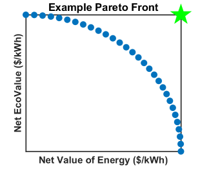
\includegraphics[width=0.9\linewidth]{figs/img0038.png}
	
\end{frame}


\begin{frame}
	\frametitle{Electricity Markets by Region}
	
	\centering
	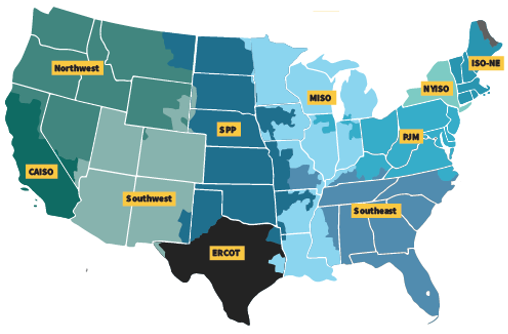
\includegraphics[width=0.9\linewidth]{figs/img0039.png}
	
	{\footnotesize Image: FERC}
	no capacity markets
	
\end{frame}


\begin{frame}
	\frametitle{What effects are important?}
	
	\centering
	\begin{itemize}
		\item Utilize other studies for a first-pass model
	\end{itemize}
	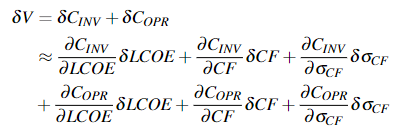
\includegraphics[width=0.9\linewidth]{figs/img0040.png}
	\begin{tabular}{|l|l|l|l|} \hline
		Study            & 1 - Coe et al.                & 2 - EVOLVE             & 3 - de Faria et al. \\ \hline
		Geographic Scope & California                    & UK (Ireland, Portugal) & North Carolina      \\ \hline
		Model            & Simplified Capacity Expansion & Economic Dispatch      & Capacity Expansion  \\ \hline
		Parameters       & LCOE, CF                      & Capacity               & σCF                \\ \hline
		Cost             & Investment                    & Operating              & Investment          \\ \hline
	\end{tabular}
	
\end{frame}


\begin{frame}
	\frametitle{What effects are important? Capacity cost >> operating cost}
	
	\centering
	\begin{itemize}
		\item Operating costs maximum 4% of total cost, so neglect in future work
		\item Future work: use capacity expansion model to derive weights
	\end{itemize}
	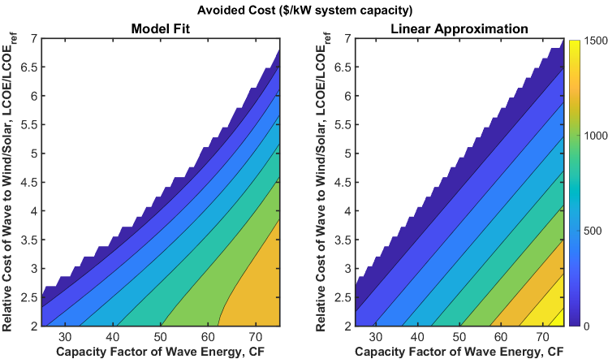
\includegraphics[width=0.9\linewidth]{figs/img0041.png}
	
	{\footnotesize McCabe, Dietrich, Liu, and Haji, 2023.}
	
\end{frame}


\begin{frame}
	\frametitle{Loop Structures}
	\begin{tabular}{|l|l|l|} \hline
		                                 & LP Computational Cost & NLP Computational Cost \\ \hline
		Current: Reduced order model + lookup table & 4D sweep: 104 combos
		1 min each
		Total: 7 days & 100 iterations
		13 function calls per iteration
		50 ms per function call
		Total: 1 minute  \\ \hline
		Possible: price taker assumption & 1 min                 & 1 min                  \\ \hline
		Possible: CEM in the loop        & None                  & 100 iterations         
		13 function calls per iteration
		1 minute per function call
		Total: 20 hours  \\ \hline
		Possible: single huge CEM        & 10 min                & 8D sweep = 108 combos  
		50 ms per function call
		Total: 10 weeks  \\ \hline
	\end{tabular}
	
	
\end{frame}


\begin{frame}
	\frametitle{Proposed Process}
	\begin{itemize}
		\item Run CEM with no WECs
		\item Consolidate results w/ ocean data to get marginal cost and carbon vs Hs, Te
		\item Run design optimization to max WEC net value with price taker assumption
		\item Run design optimization to max WEC net value with CEM in the loop
		\item Run design optimization to max system value with CEM in the loop
		\item Repeat 1-5 for different grid conditions (location, electrification)
		\item No ROM, so no RQ4 (how does power matrix affect system value?)
	\end{itemize}
\end{frame}


\begin{frame}
	\frametitle{Journal Summary}
	\begin{tabular}{|l|l|l|l|l|} \hline
		#                       & Title                                                                                                             & Target Journal             & Target submission & Status         \\ \hline
		J1 MDOcean modeling     & Development, Validation, and Benchmarking of a Multidisciplinary Semi-Analytical Model for Wave Energy Converters & Applied Ocean Research     & October 2025      & Editing (101p) \\ \hline
		J2 MDOcean optimization & Leveraging Multidisciplinary Design Optimization to Advance Wave Energy Converter Viability                       & Renewable Energy           & December 2025     & Editing (128p) \\ \hline
		J3 MEEM                 & Numerics of the matched eigenfunction method for computing wave forces on concentric bodies                       & Journal of Fluid Mechanics & December 2025     & Drafting       \\ \hline
		J4 DECIDER              & TBD                                                                                                               & Applied Energy             & May 2025          & Working        \\ \hline
	\end{tabular}
	
	
\end{frame}


\begin{frame}
	\frametitle{Publication Plan}
	\begin{itemize}
		\item Analytical modeling of WECs
		      \begin{itemize}
		      	\item Hydrodynamics: matched eigenfunction expansion method C6, C7, J3
		      	\item Dynamics: constraints and nonlinearities via describing functions C9, J1
		      	\item Structures: stiffened plate model J1
		      	\item Synthesis, validation, and benchmarking C10, C11, J1
		      \end{itemize}
		\item Design optimization of WECs
		      \begin{itemize}
		      	\item Design for cost: multidisciplinary design optimization C1, C10, J2
		      	\item Design for value: integrated capacity expansion model C2, C5, C11, J4
		      \end{itemize}
		      
		\item Side projects (as co-author):
		\item Aquaculture C3, C4
		\item WEC prototyping C13, J5
		\item Carbon sequestration C8, C12
		      
		\item So far: 13 conferences
		\item Future: 5 journals
	\end{itemize}
	
\end{frame}


\begin{frame}
	\frametitle{Publications}
	\begin{itemize}
		\item McCabe, Khanal, and Haji, “Open-source toolbox for semi-analytical hydrodynamic coefficients via the matched eigenfunction expansion method,“ August 2024, UMERC+METS Conference, Duluth MN.
		\item Best, Khanal, McCabe, Jiang, Treacy, and Haji, “OpenFLASH: An open-source flexible library for analytical and semi-analytical hydrodynamics calculations,” in review for Journal of Open-Source Software.
		\item McCabe, Khanal, Bimali, Lo, Treacy, and Haji, “Numerics of the matched eigenfunction method for computing wave forces on concentric bodies,” in preparation for submission to Journal of Fluid Mechanics.
	\end{itemize}
\end{frame}


\begin{frame}
	\frametitle{Capacity Expansion Model: Global Sensitivity Analysis}
	\begin{itemize}
		\item State of world sweep
		\item - Demand scenario
		\item - Carbon constraint
		\item - Wave data year
		\item - Location of all data
		      
		\item Design sweep
		\item - D, R, ��m from
		\item force sat paper
		\item - Mode (gain,
		\item directionality,
		\item Z(ꞷ) shape)
		\item - Cost
		      
		\item GenX CEM run for 2030, 40, 50
		      
		\item Capacity wave built
		\item System cost avoided
		\item Carbon emissions avoided
		      
		\item Surrogate model, robustness evaluation
		      
		\item Sweep strategy: full factorial, but one-at-a-time on wave data year
	\end{itemize}
	
\end{frame}


\begin{frame}
	\frametitle{Question 2 (Jacob): CEM Econ Interaction}
	\begin{itemize}
		\item CEM
		      
		\item Cost model
		      
		\item Design
		      
		\item Max cost for viability
		      
		\item Modeled cost
		      
		\item Cost leftover for unmodeled components
		      
		\item Ignore CEM outputs, never flat, no cost assumption
		      
		\item CEM
		      
		\item Cost model
		      
		\item Design
		      
		\item Avoided system cost for each WEC cost
		      
		\item Modeled cost
		      
		\item Cost estimate for unmodeled components
		      
		\item Uses CEM outputs, flat, cost assumption
		      
		\item Avoided system cost
	\end{itemize}
	
\end{frame}


\begin{frame}
	\frametitle{Describing Functions}
	
	\centering
	\begin{itemize}
		\item Analytical expression for fundamental harmonic
	\end{itemize}
	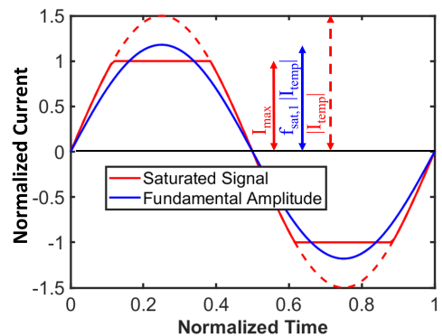
\includegraphics[width=0.9\linewidth]{figs/img0042.png}
	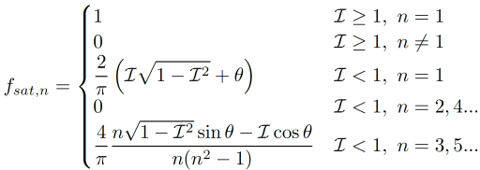
\includegraphics[width=0.9\linewidth]{figs/img0043.png}
	
	{\footnotesize McCabe and Haji, “Force-Limited Control of Wave Energy Converters using a Describing Function Linearization,“ September 2024, IFAC CAMS Conference, Blacksburg VA.}
	
\end{frame}


\begin{frame}
	\frametitle{MEEM Computational Results: Runtime, Convergence}
	
	\centering
	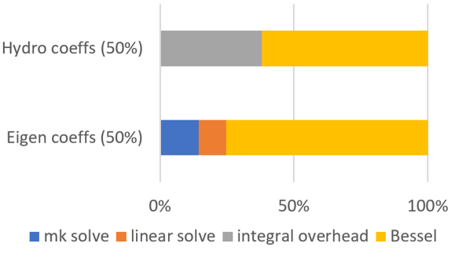
\includegraphics[width=0.9\linewidth]{figs/img0044.png}
	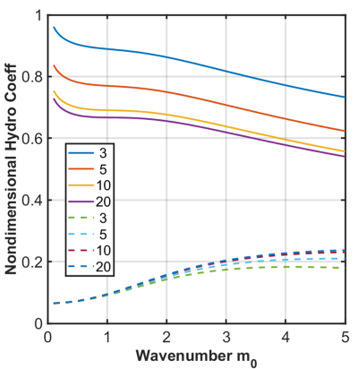
\includegraphics[width=0.9\linewidth]{figs/img0045.png}
	
\end{frame}


\begin{frame}
	\frametitle{MEEM equations and setup}
	
	\centering
	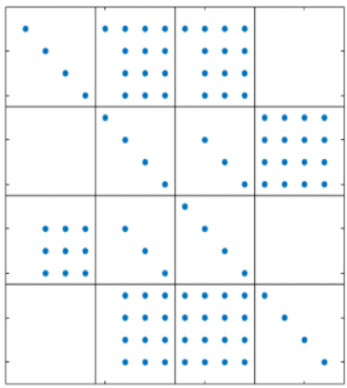
\includegraphics[width=0.9\linewidth]{figs/img0046.png}
	\begin{itemize}
		\item A-matrix sparsity for N=M=K=4
		      
		\item N
		      
		\item M
		      
		\item M
		      
		\item K
		      
		\item N          M         M          K
	\end{itemize}
	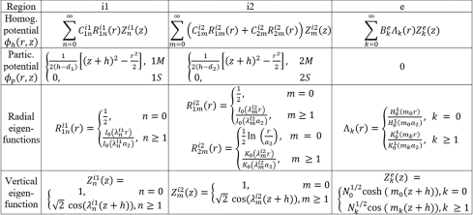
\includegraphics[width=0.9\linewidth]{figs/img0047.png}
	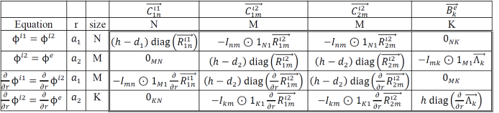
\includegraphics[width=0.9\linewidth]{figs/img0048.png}
	
\end{frame}


\begin{frame}
	\frametitle{Visualizing Amplitude Constraints on Smith Chart}
	
	\centering
	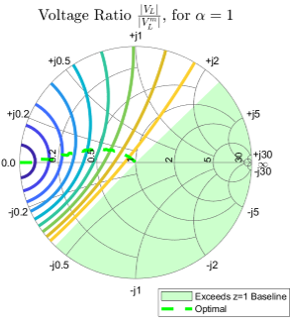
\includegraphics[width=0.9\linewidth]{figs/img0049.png}
	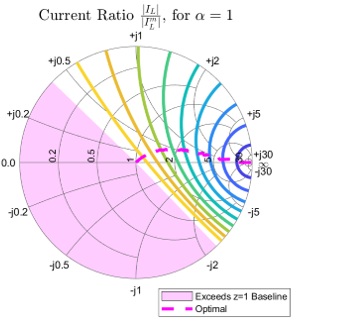
\includegraphics[width=0.9\linewidth]{figs/img0050.png}
	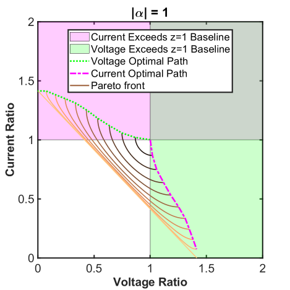
\includegraphics[width=0.9\linewidth]{figs/img0051.png}
	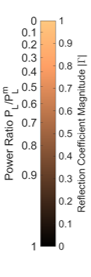
\includegraphics[width=0.9\linewidth]{figs/img0052.png}
	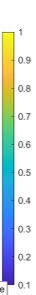
\includegraphics[width=0.9\linewidth]{figs/img0053.png}
	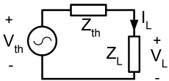
\includegraphics[width=0.9\linewidth]{figs/img0054.png}
	
\end{frame}


\begin{frame}
	\frametitle{Describing Function Block Diagram}
	
	\centering
	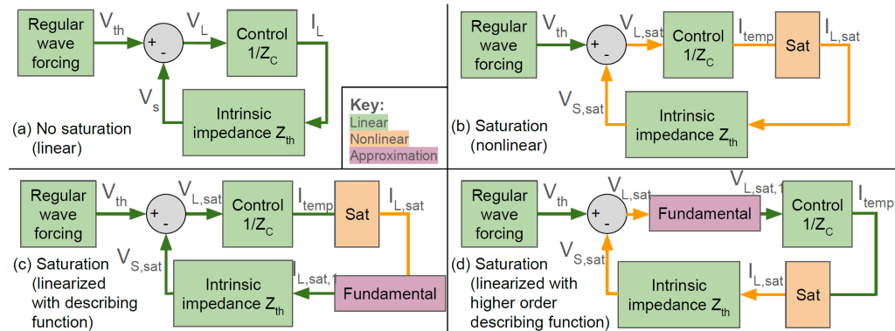
\includegraphics[width=0.9\linewidth]{figs/img0055.png}
	
\end{frame}


\begin{frame}
	\frametitle{A-Exam Slides}
\end{frame}


\begin{frame}
	\frametitle{Agenda}
	\begin{itemize}
		\item Motivation
		\item Techno-Economic and Environmental Metrics
		      \begin{itemize}
		      	\item Metric selection
		      	\item Metric weighting
		      	\item Optimization framework
		      \end{itemize}
		\item Design Optimization
		      \begin{itemize}
		      	\item V1 formulation and results
		      	\item V2 formulation
		      	\item V3 concept
		      \end{itemize}
		\item Conclusion
	\end{itemize}
\end{frame}


\begin{frame}
	\frametitle{Future Design Optimization Features}
	\begin{tabular}{|l|l|l|l|l|l|} \hline
		Version & Hydro Coefficients             & Controls                                             & Storage & Objective              & Architecture \\ \hline
		V1      & Long wave approximation        & Same for all sea states, linear with saturation      & No      & LCOE and cv            & RM3 only     \\ \hline
		V2      & Analytical PDE solution        & Different for each sea state, linear with saturation & Yes     & LCOE and cv            & RM3 only     \\ \hline
		V3      & Boundary element method solver & WecOptTool, nonlinear                                & Yes     & NVOE and net eco-value & Various      \\ \hline
	\end{tabular}
	
	
\end{frame}


\begin{frame}
	\frametitle{V2 - Improved Analytical Hydrodynamic Coefficients}
	
	\centering
	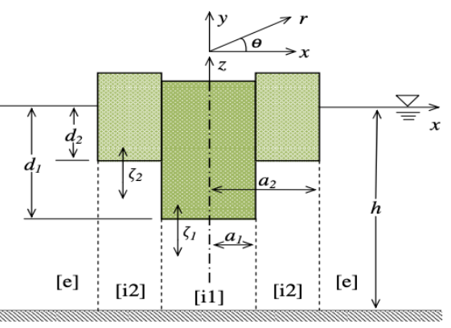
\includegraphics[width=0.9\linewidth]{figs/img0056.png}
	\begin{itemize}
		\item Laplace’s equation
		\item PDE boundary conditions
		\item Matched eigenfunction method
		\item Symbolic, differentiable
		\item Faster than BEM, no approximations
	\end{itemize}
	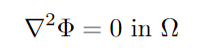
\includegraphics[width=0.9\linewidth]{figs/img0057.png}
	
	{\footnotesize Chau and Yeung, 2010.}
	
\end{frame}


\begin{frame}
	\frametitle{V2 - Energy Storage}
	\begin{itemize}
		\item Can WEC design reduce power variability more effectively than energy storage?
		\item Generate power probability density function without storage
		\item Account for storage with a given power limit
		\item Account for storage with a given energy capacity
		\item Calculate the impact on cost and power variation
		\item Compare to pareto front without storage
		      
		\item McCabe, Murphy, and Haji, 2022.
	\end{itemize}
	
\end{frame}


\begin{frame}
	\frametitle{V3 Concept}
	
	\centering
	\begin{itemize}
		\item Bi-level optimization, enhanced control co-design
	\end{itemize}
	
\includegraphics[width=0.9\linewidth]{figs/img0058.png}
	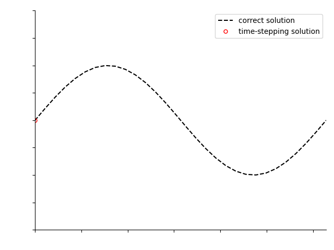
\includegraphics[width=0.9\linewidth]{figs/img0059.png}
	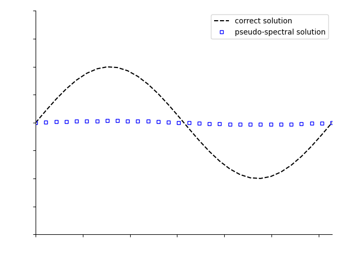
\includegraphics[width=0.9\linewidth]{figs/img0060.png}
	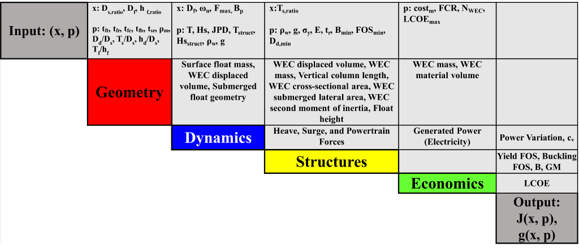
\includegraphics[width=0.9\linewidth]{figs/img0061.png}
	\begin{itemize}
		\item Internal optimization with WecOptTool
		\item DV: WEC response and powertrain force harmonics
		\item Objective: power (convex) or cost (nonconvex)
		      
		\item + Environment
	\end{itemize}
	
\end{frame}


\begin{frame}
	\frametitle{Agenda}
	\begin{itemize}
		\item Motivation
		\item Techno-Economic and Environmental Metrics
		      \begin{itemize}
		      	\item Metric selection
		      	\item Metric weighting
		      	\item Optimization framework
		      \end{itemize}
		\item Design Optimization
		      \begin{itemize}
		      	\item V1 formulation and results
		      	\item V2 formulation
		      	\item V3 concept
		      \end{itemize}
		\item Conclusion
	\end{itemize}
\end{frame}


\begin{frame}
	\frametitle{Conference Papers and Presentations}
	\begin{itemize}
		\item Khanal, McCabe, and Haji, “Gradient-based Design Optimization of Concentric Cylindrical Offshore Structures,” 2023. SIAM Conference on Optimization. Accepted.
		\item McCabe, Dietrich, Liu, and Haji, 2023. “System Level Techno-Economic and Environmental Design Optimization for Ocean Wave Energy.” ASME IDETC-CIE: Design Automation Conference. In Press.
		\item Hasankhani, McCabe, Ewig, Won, and Haji, 2023. “Design of a Wave-Powered Aquaculture Farm,” International Ocean and Polar Engineering Conference. In Press.
		\item Hasankhani, Ewig, McCabe, Won, and Haji, 2023. “Marine Spatial Planning of a Wave-Powered Offshore Aquaculture Farm in the Northeast U.S.” IEEE Oceans Conference – Limerick. In Press.
		\item McCabe and Haji, 2022, “Value Metrics and Global Impact Potential of Wave Energy,” University Marine Energy Research Community Conference.
		\item McCabe, Murphy, and Haji, 2022, “Multidisciplinary Optimization to Reduce Cost and Power Variation of a Wave Energy Converter,” ASME IDETC-CIE: Design Automation Conference. https://doi.org/10.1115/DETC2022-90227.
	\end{itemize}
\end{frame}


\begin{frame}
	\frametitle{Backup Slides}
\end{frame}


\begin{frame}
	\frametitle{Metric Weighting - Grid Scale - Study 1}
	
	\centering
	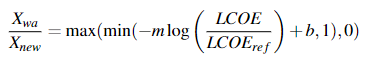
\includegraphics[width=0.9\linewidth]{figs/img0062.png}
	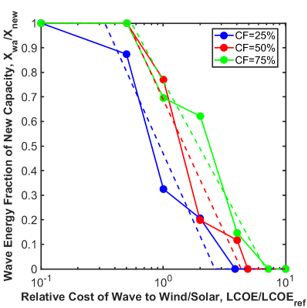
\includegraphics[width=0.9\linewidth]{figs/img0063.png}
	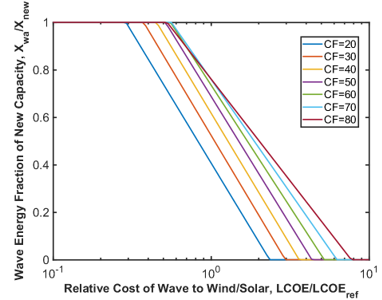
\includegraphics[width=0.9\linewidth]{figs/img0064.png}
	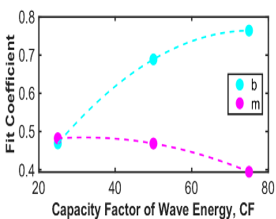
\includegraphics[width=0.9\linewidth]{figs/img0065.png}
	
\end{frame}


\begin{frame}
	\frametitle{Metric Weighting - Grid Scale - Study 2}
	
	\centering
	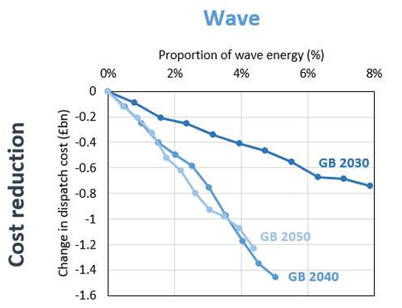
\includegraphics[width=0.9\linewidth]{figs/img0066.png}
	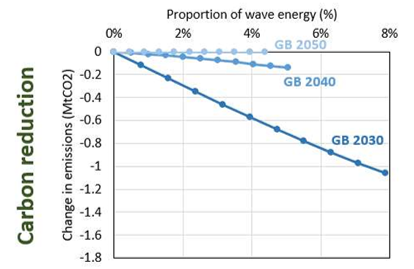
\includegraphics[width=0.9\linewidth]{figs/img0067.png}
	
\end{frame}


\begin{frame}
	\frametitle{Metric Weighting - Grid Scale - Study 3}
	
	\centering
	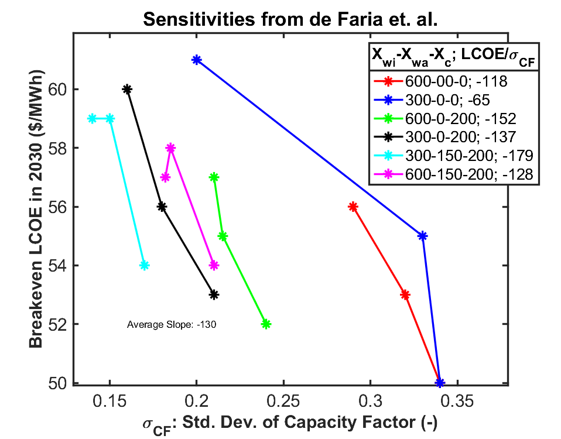
\includegraphics[width=0.9\linewidth]{figs/img0068.png}
	
\end{frame}


\begin{frame}
	\frametitle{Metric Selection}
	\begin{tabular}{|l|l|l|l|l|l|} \hline
		Temporal value & Consistency                       & Technical                                & Economic                         & Environmental               & Operational                       \\ \hline
		Availability   & Coefficient of variation of power & Capture width (ratio)                    & Levelized cost (value) of energy & Net EcoCosts                & Manufacturability                 \\ \hline
		Persistence    & Capacity factor                   & Technology readiness (performance) level & Payback period                   & Global warming potential    & Deployability and maintainability \\ \hline
		Versatility    & Force peak to average ratio       & Hydrodynamic performance quality         & Internal rate of return          & Energy return on investment & Robustness to uncertainty         \\ \hline
	\end{tabular}
	
	
\end{frame}


\begin{frame}
	\frametitle{Optimization - Dealing with Categorical Variables}
	\begin{itemize}
		\item Separate gradient-based optimization for each integer combination
		\item Nested gradient-based solver inside a heuristic solver
		\item MINLP solver: AMIEGO, APOPT, Baron, Couenne, Bonmin, mindtPy
		      \begin{itemize}
		      	\item Only AMIEGO has been used with OpenMDAO
		      	\item Others available from pyomo and Gekko packages
		      \end{itemize}
		      
		\item Decreasing computational cost
		\item Increasing implementation complexity
	\end{itemize}
	
\end{frame}


\begin{frame}
	\frametitle{Optimization - Making it Multiobjective}
	\begin{itemize}
		\item Construct the pareto front with a sequence of single-objective optimizations
		      \begin{itemize}
		      	\item Normal boundary intersection method to generate evenly spaced points for nonconvex part of the pareto front
		      \end{itemize}
		\item Use the above method to generate a few points, and use those as initial population in MOGA or similar
		\item Fancy research algorithms for inherently gradient-based multiobjective optimization
		      \begin{itemize}
		      	\item Not available in python packages
		      \end{itemize}
		      
		\item Decreasing computational cost
		\item Increasing implementation complexity
	\end{itemize}
	
\end{frame}


\begin{frame}
	\frametitle{Optimization Convergence and Global Minimum}
	\begin{itemize}
		\item 100 random initial designs
		\item Of the ~40% that converged with the KKT conditions satisfied, how many found the best local optimum?
	\end{itemize}
	\begin{tabular}{|l|l|} \hline
		LCOE minimization & 67%   \\ \hline
		Cv minimization   & 98%   \\ \hline
	\end{tabular}
	
	
\end{frame}


\begin{frame}
	\frametitle{Modeling and Simulation}
	
	\centering
	\begin{itemize}
		\item Device Power Capability      *	     Site Wave Data  	  =	      Power Production
	\end{itemize}
	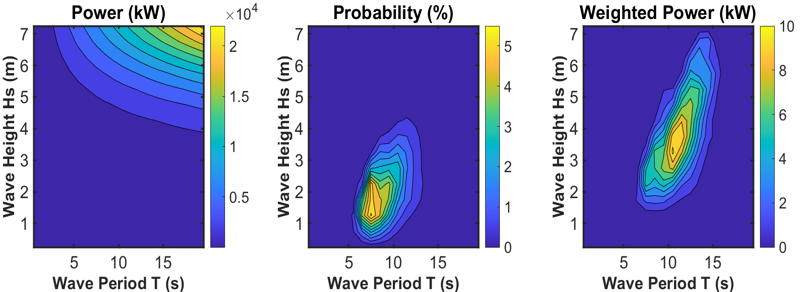
\includegraphics[width=0.9\linewidth]{figs/img0069.png}
	\begin{itemize}
		\item JPD for Humboldt, CA
		      
		\item From Simulation
	\end{itemize}
\end{frame}


\begin{frame}
	\frametitle{Power Distribution Comparison}
	
	\centering
	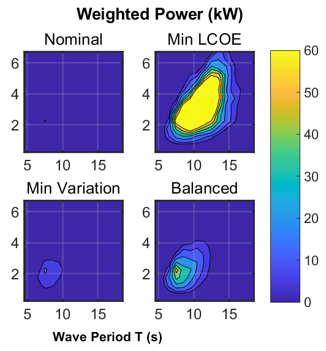
\includegraphics[width=0.9\linewidth]{figs/img0070.png}
	
\end{frame}


\begin{frame}
	\frametitle{Matched Eigenfunction Method - Boundary Value}
	
	\centering
	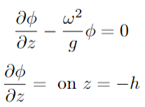
\includegraphics[width=0.9\linewidth]{figs/img0071.png}
	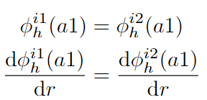
\includegraphics[width=0.9\linewidth]{figs/img0072.png}
	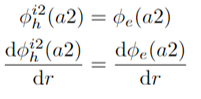
\includegraphics[width=0.9\linewidth]{figs/img0073.png}
	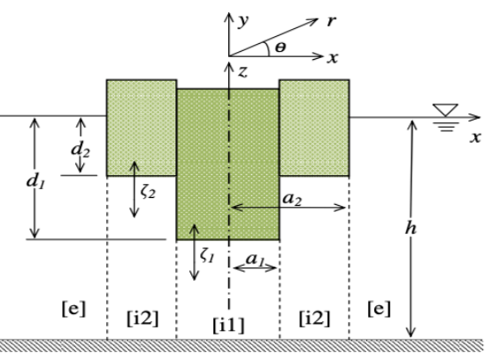
\includegraphics[width=0.9\linewidth]{figs/img0074.png}
	
\end{frame}



\begin{frame}
	\frametitle{Conference Papers and Presentations}
	\begin{itemize}
		\item Khanal, McCabe, and Haji, “Gradient-based Design Optimization of Concentric Cylindrical Offshore Structures,” 2023. SIAM Conference on Optimization. Accepted.
		\item {\footnotesize\color{gray}\cite{mccabe_system_2023}}
		\item Hasankhani, McCabe, Ewig, Won, and Haji, 2023. “Design of a Wave-Powered Aquaculture Farm,” International Ocean and Polar Engineering Conference. In Press.
		\item Hasankhani, Ewig, McCabe, Won, and Haji, 2023. “Marine Spatial Planning of a Wave-Powered Offshore Aquaculture Farm in the Northeast U.S.” IEEE Oceans Conference – Limerick. In Press.
		\item {\footnotesize\color{gray}\cite{mccabe_multidisciplinary_2022}}
		\item {\footnotesize\color{gray}\cite{mccabe_multidisciplinary_2022}}
	\end{itemize}
\end{frame}


\begin{frame}
	\frametitle{Backup Slides}
\end{frame}


\begin{frame}
	\frametitle{Metric Weighting - Grid Scale - Study 1}
	
	\centering
	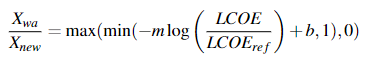
\includegraphics[width=0.9\linewidth]{figs/img0062.png}
	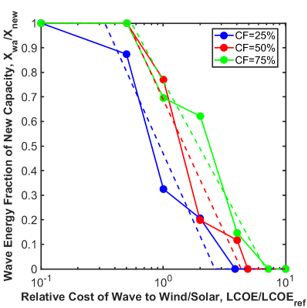
\includegraphics[width=0.9\linewidth]{figs/img0063.png}
	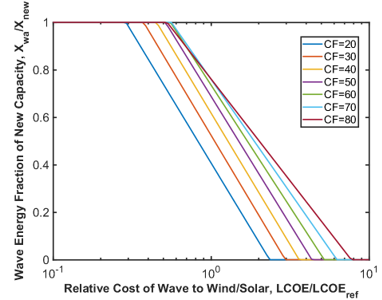
\includegraphics[width=0.9\linewidth]{figs/img0064.png}
	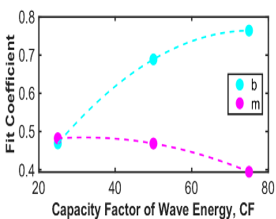
\includegraphics[width=0.9\linewidth]{figs/img0065.png}
	
\end{frame}


\begin{frame}
	\frametitle{Metric Weighting - Grid Scale - Study 2}
	
	\centering
	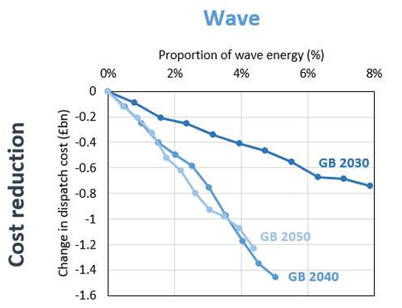
\includegraphics[width=0.9\linewidth]{figs/img0066.png}
	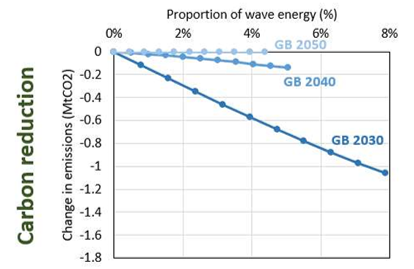
\includegraphics[width=0.9\linewidth]{figs/img0067.png}
	
\end{frame}


\begin{frame}
	\frametitle{Metric Weighting - Grid Scale - Study 3}
	
	\centering
	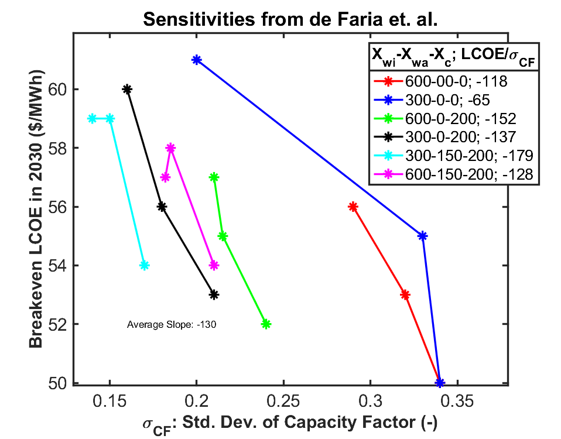
\includegraphics[width=0.9\linewidth]{figs/img0068.png}
	
\end{frame}


\begin{frame}
	\frametitle{Metric Selection}
	\begin{tabular}{|l|l|l|l|l|l|} \hline
		Temporal value & Consistency                       & Technical                                & Economic                         & Environmental               & Operational                       \\ \hline
		Availability   & Coefficient of variation of power & Capture width (ratio)                    & Levelized cost (value) of energy & Net EcoCosts                & Manufacturability                 \\ \hline
		Persistence    & Capacity factor                   & Technology readiness (performance) level & Payback period                   & Global warming potential    & Deployability and maintainability \\ \hline
		Versatility    & Force peak to average ratio       & Hydrodynamic performance quality         & Internal rate of return          & Energy return on investment & Robustness to uncertainty         \\ \hline
	\end{tabular}
	
	
\end{frame}


\begin{frame}
	\frametitle{Optimization - Dealing with Categorical Variables}
	\begin{itemize}
		\item Separate gradient-based optimization for each integer combination
		\item Nested gradient-based solver inside a heuristic solver
		\item MINLP solver: AMIEGO, APOPT, Baron, Couenne, Bonmin, mindtPy
		      \begin{itemize}
		      	\item Only AMIEGO has been used with OpenMDAO
		      	\item Others available from pyomo and Gekko packages
		      \end{itemize}
		      
		\item Decreasing computational cost
		\item Increasing implementation complexity
	\end{itemize}
	
\end{frame}


\begin{frame}
	\frametitle{Optimization - Making it Multiobjective}
	\begin{itemize}
		\item Construct the pareto front with a sequence of single-objective optimizations
		      \begin{itemize}
		      	\item Normal boundary intersection method to generate evenly spaced points for nonconvex part of the pareto front
		      \end{itemize}
		\item Use the above method to generate a few points, and use those as initial population in MOGA or similar
		\item Fancy research algorithms for inherently gradient-based multiobjective optimization
		      \begin{itemize}
		      	\item Not available in python packages
		      \end{itemize}
		      
		\item Decreasing computational cost
		\item Increasing implementation complexity
	\end{itemize}
	
\end{frame}


\begin{frame}
	\frametitle{Optimization Convergence and Global Minimum}
	\begin{itemize}
		\item 100 random initial designs
		\item Of the ~40\% that converged with the KKT conditions satisfied, how many found the best local optimum?
	\end{itemize}
	\begin{tabular}{|l|l|} \hline
		LCOE minimization & 67\% \\ \hline
		Cv minimization   & 98\% \\ \hline
	\end{tabular}
	
	
\end{frame}


\begin{frame}
	\frametitle{Modeling and Simulation}
	
	\centering
	\begin{itemize}
		\item Device Power Capability      *	     Site Wave Data  	  =	      Power Production
	\end{itemize}
	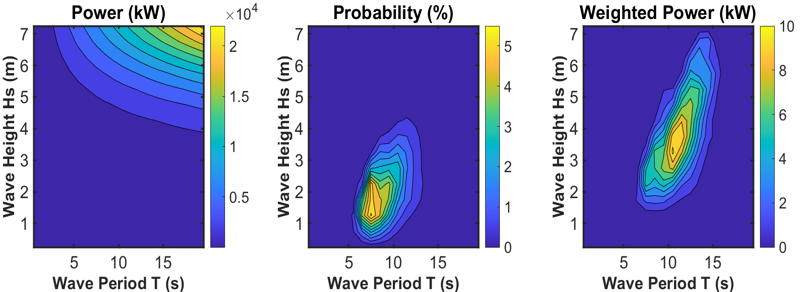
\includegraphics[width=0.9\linewidth]{figs/img0069.png}
	\begin{itemize}
		\item JPD for Humboldt, CA
		      
		\item From Simulation
	\end{itemize}
\end{frame}


\begin{frame}
	\frametitle{Power Distribution Comparison}
	
	\centering
	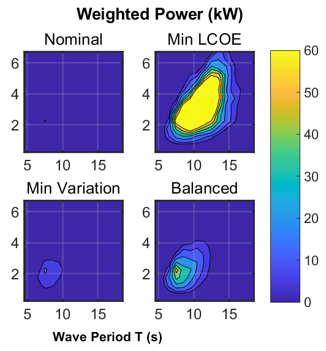
\includegraphics[width=0.9\linewidth]{figs/img0070.png}
	
\end{frame}


\begin{frame}
	\frametitle{Matched Eigenfunction Method - Boundary Value}
	
	\centering
	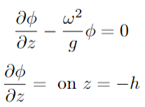
\includegraphics[width=0.9\linewidth]{figs/img0071.png}
	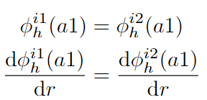
\includegraphics[width=0.9\linewidth]{figs/img0072.png}
	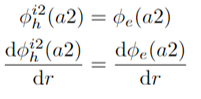
\includegraphics[width=0.9\linewidth]{figs/img0073.png}
	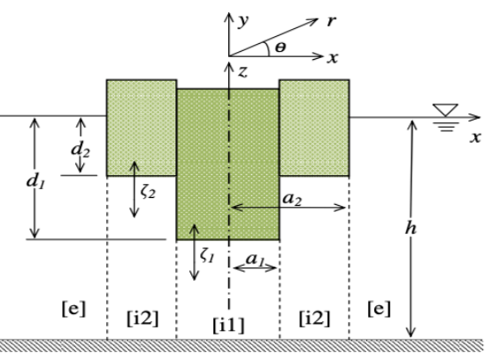
\includegraphics[width=0.9\linewidth]{figs/img0074.png}
	
\end{frame}